\section{Desgin}%
\label{sec:desgin}

\iffalse
这一张将写本系统是如何设计的,主要内容分为两部分:一部分是如何hook。另外一部分是如何实现对各种数据结构的保护。

本文的特权特指就是内存管理,管理VMCS的原因就是里边含有EPTP,其余的域并不进行保护。

那么文章的核心就是剥夺了VMM管理物理内存的权限,这就是HyperPS的P的内容。
那么针对这一特点,这一思路,设计要怎么写。
要说明如下的几个问题:1. 如何分离权限,即VMM管理内存都是靠什么实现的,特权的实现途径是啥,怎么将这些特权分离。这里要写出两个东西:1.1 原本的VMM对内存管理的相关函数被Hook,所有的操作都无法在VMM中实施,即完成了HOOK。1.2 为了防止攻击者直接修改EPT paging structure,这就是将EPT从常规的空间中移除。
这两个点要顺序换过来,先写移除,再写hook。
2. 第二要写怎么实现保护,在hook完成后,剥离了VMM对物理内存的管理,HyperPS是如何实现对内存的管理的。这里要假如关于缺页中断的相关内容,怎么处理EPT异常,也要处理新建EPT的内容,也要包括不同虚拟机的映射关系,也要绑定EPT与VM的关系,不允许VM和VMM更改EPTP内容。

上面的1 2就是两段的内容,首先要给出一个overview,讲整个框架的结构。

##################
开头内容中文初稿
##################
这一节,我们首先提出我们的HyperPS,我们详细描述HyperPS的构成组件。然后我们详细阐述了HyperPS是如何剥离原VMM对内存的管理权限的。最后我们提出HyperPS是如何实现对内存的保护,从而实现保护虚拟机的运行以抵御一个受危害的VMM。
讲HyperPS如何实现对物理内存的管理。
\fi
In this section, we first propose the architecture of HyperPS. Then, in the following subsection, we elaborate on how HyperPS stripped the compromised HostOS kernel's privilege of managing guest VM's memory and the physical memory. Finally, we propose how HyperPS manages the guest VM's memory and physical memory to resist the compromised HostOS/Hypervisor.


\subsection{HyperPS Overview}%
\label{sub:hyperps_overview}

% 首先一句话说明HyperPS要做什么,然后Figure depict the details on the architecture of HyperPS.
% As shown in Figure, 我们创造了一个同层隔离空间用于履行原本属于compromised HostOS的管理虚拟机物理内存的权力。


We present HyperPS to protect guest virtual machines against compromised hypervisor. In virtualization environment, the hyperivor deprivileges the guest VM’s kernel and interposes all interactions between guest VMs and the physical memory. Neither isolation between VMs nor virtual-physical mapping relationships in a VM will inevitable be tamperred if the hypervisor is compromised. HyperPS, thus, deprives the hypervisor of privileges on managing physical memory.


Figure \ref{fig:design} depicts the details on the architecture of HyperPS. 
Firstly, as shown in Figure \ref{fig:design}, we create a delicate kernel-level secure and isolated execution space, called HyperPS Space, to inherit privileges of managing physical memory that originally belonged to the compromised hypervisor. 
Original funtions about physical memory management in the compromised hypervisor, such as EPT operations and EPTP switching operations in VMCS operations, are hooked into the HyperPS space. 
However, there are still some cases where attackers subvert memory management data structures by using regular memory access, attackers can also bypass the hooked functions by introducing new malicious VMX assembly code. HyperPS, in consideration of these cases, removed VMCS and EPT from the original hypervisor space and placed them in the HyperPS space. 
% For cases where attackers subvert memory management data structures by using regular memory access, and cases where attackers bypass the hooked functions by introducing new malicious VMX assembly code
% use regular memory access to tamper with
% For cases where an attacker uses regular memory access or newly introduced malicious VMX assembly code to bypass the hooked functions and tamper with the relevant memory management data structures, HyperPS removed VMCS and EPT, which are crucial to virtualization, from the original hypervisor space and places them in the HyperPS Space.
Secondly, in the HyperPS space, we introduce a new data structure, called Physical Page Tag Table (PPTT), to tag the mapping relations between the physical frames and the virtual machines. With the help of this data structure, even if an attacker tampers EPT Paging Structures with malicious value through a legal function, HyperPS can still effectively detect such attack and resist it.
Lastly, Switch Gate is the only interface between the kernel space and the HyperPS space.

%FIXME 图中的内容添加虚拟机退出的线,removed的字段加粗 pptt是表 修改成表的形式

\begin{figure}[htpb]
    \centering
    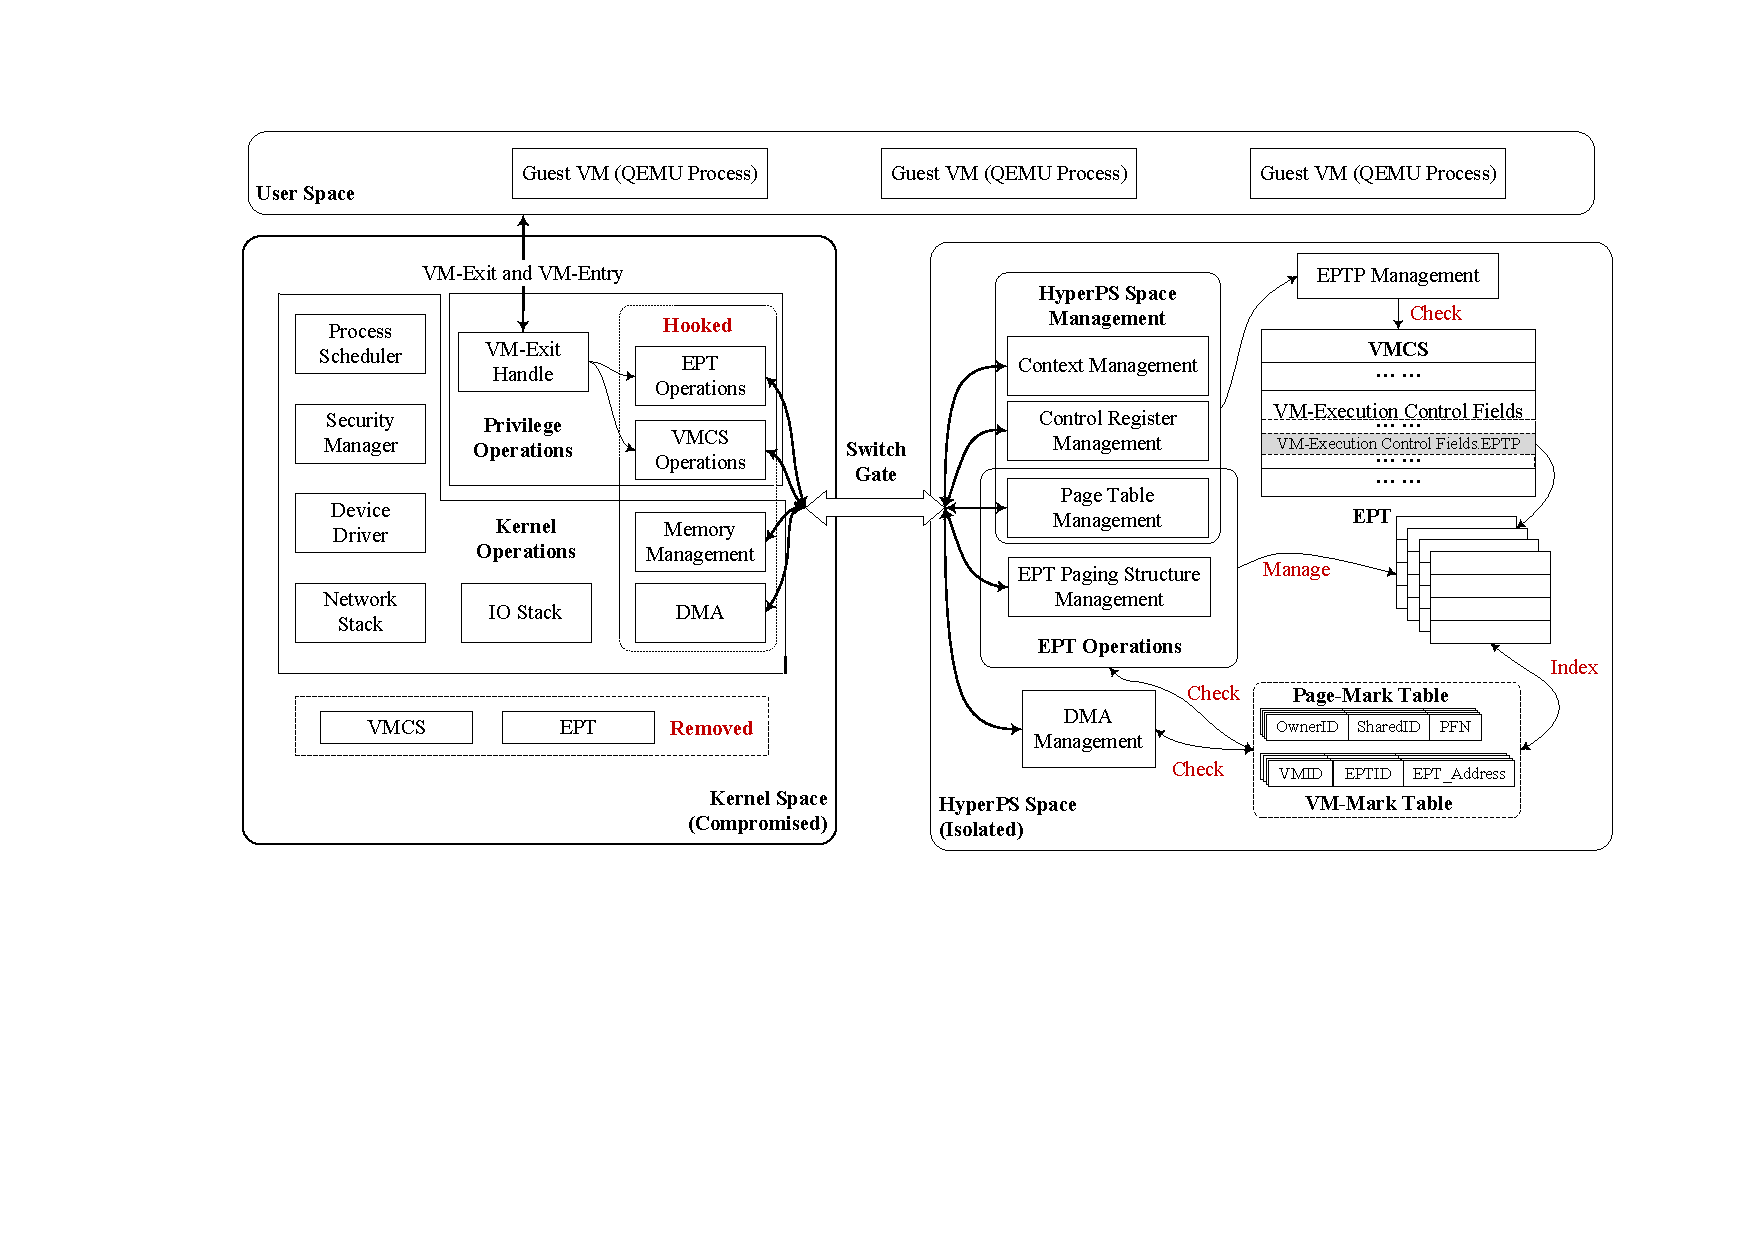
\includegraphics[width=0.9\linewidth]{IMG/design.pdf}
    \caption{HyperPS Architecture}%
    \label{fig:design}
\end{figure}



\iffalse
那么文章的核心就是剥夺了VMM管理物理内存的权限,这就是HyperPS的P的内容。
那么针对这一特点,这一思路,设计要怎么写。
要说明如下的几个问题:1. 如何分离权限,即VMM管理内存都是靠什么实现的,特权的实现途径是啥,怎么将这些特权分离。这里要写出两个东西:1.1 原本的VMM对内存管理的相关函数被Hook,所有的操作都无法在VMM中实施,即完成了HOOK。1.2 为了防止攻击者直接修改EPT paging structure,这就是将EPT从常规的空间中移除。
这两个点要顺序换过来,先写移除,再写hook。
2. 第二要写怎么实现保护,在hook完成后,剥离了VMM对物理内存的管理,HyperPS是如何实现对内存的管理的。这里要假如关于缺页中断的相关内容,怎么处理EPT异常,也要处理新建EPT的内容,也要包括不同虚拟机的映射关系,也要绑定EPT与VM的关系,不允许VM和VMM更改EPTP内容。
\fi

\subsection{Privilege Separation}%
\label{sub:privilege_separation}

\iffalse
首先要讲管理内存的权限是通过EPT实现的,要实现特权的分离,分为两步,一是将EPT从原有空间移除,使得原有的hypervisor无法直接access数据结构。第二步是对能access这些数据结构的函数进行验证。
% 将移除操作这些数据结构的逻辑。
在传统的没有HyperPS的虚拟化环境中,Hypervisor 通过EPT直接管理管理内存
这里要先讲为什么要将EPT和VMCS从原有的空间移除,然后再讲怎么移除。移除以后存在疑问,就是会造成PANIC, 如何解决,就是hook的问题,
EPT defines a layer of address translation that augments the translation of linear addresses. 
The EPT mechanism is a feature that can be used to support the virtualization of physical memory. When EPT is in use, certain addresses that would mormally be treated as physical addresses (and used to access memory) are instead trated as guest-physical addresses. Guest-physical addresses are tranlated by traversing a set of EPT paging structures to produce physical addresses that are used to access memory.
It's EPT mechanism that treat guest-physical address like a virtual address and the EPTP is the CR3.
we should write (VMWRITE) EPTP to the VMCS. 
\fi

% According to the Intel manual, the EPT mechanism is a core feature that is used to support the virtualization of physical memory.
EPT defines a layer of address translation that augments the translation of linear addresses. 
When EPT is in use, the EPT interposes all memory access between guest VMs and the physical memory. 
Certain addresses that would mormally be treated as physical addresses (and used to access memory) are instead treated as guest-physical addresses. Guest-physical addresses are translated by traversing a set of EPT paging structures to produce physical addresses that are used to access memory.
% If the hyperivor has been subverted by the attacker,
If attakers have gained control over a hypervisor, 
neither isolation between VMs nor virtual-physical mapping relationships in a VM are immune to them. 
% Attackers can modify any EPT paging structures with any values.
In this paper, HyperPS deprives the hyperivor's privileges of managing physical memory by limiting it from accessing and managing all EPTs. 
Figure \ref{fig:inter} depicts the diffrence in the VM-Exit handling between the traditional system and system with HyperPS.
\begin{figure}[htpb]
    \centering
    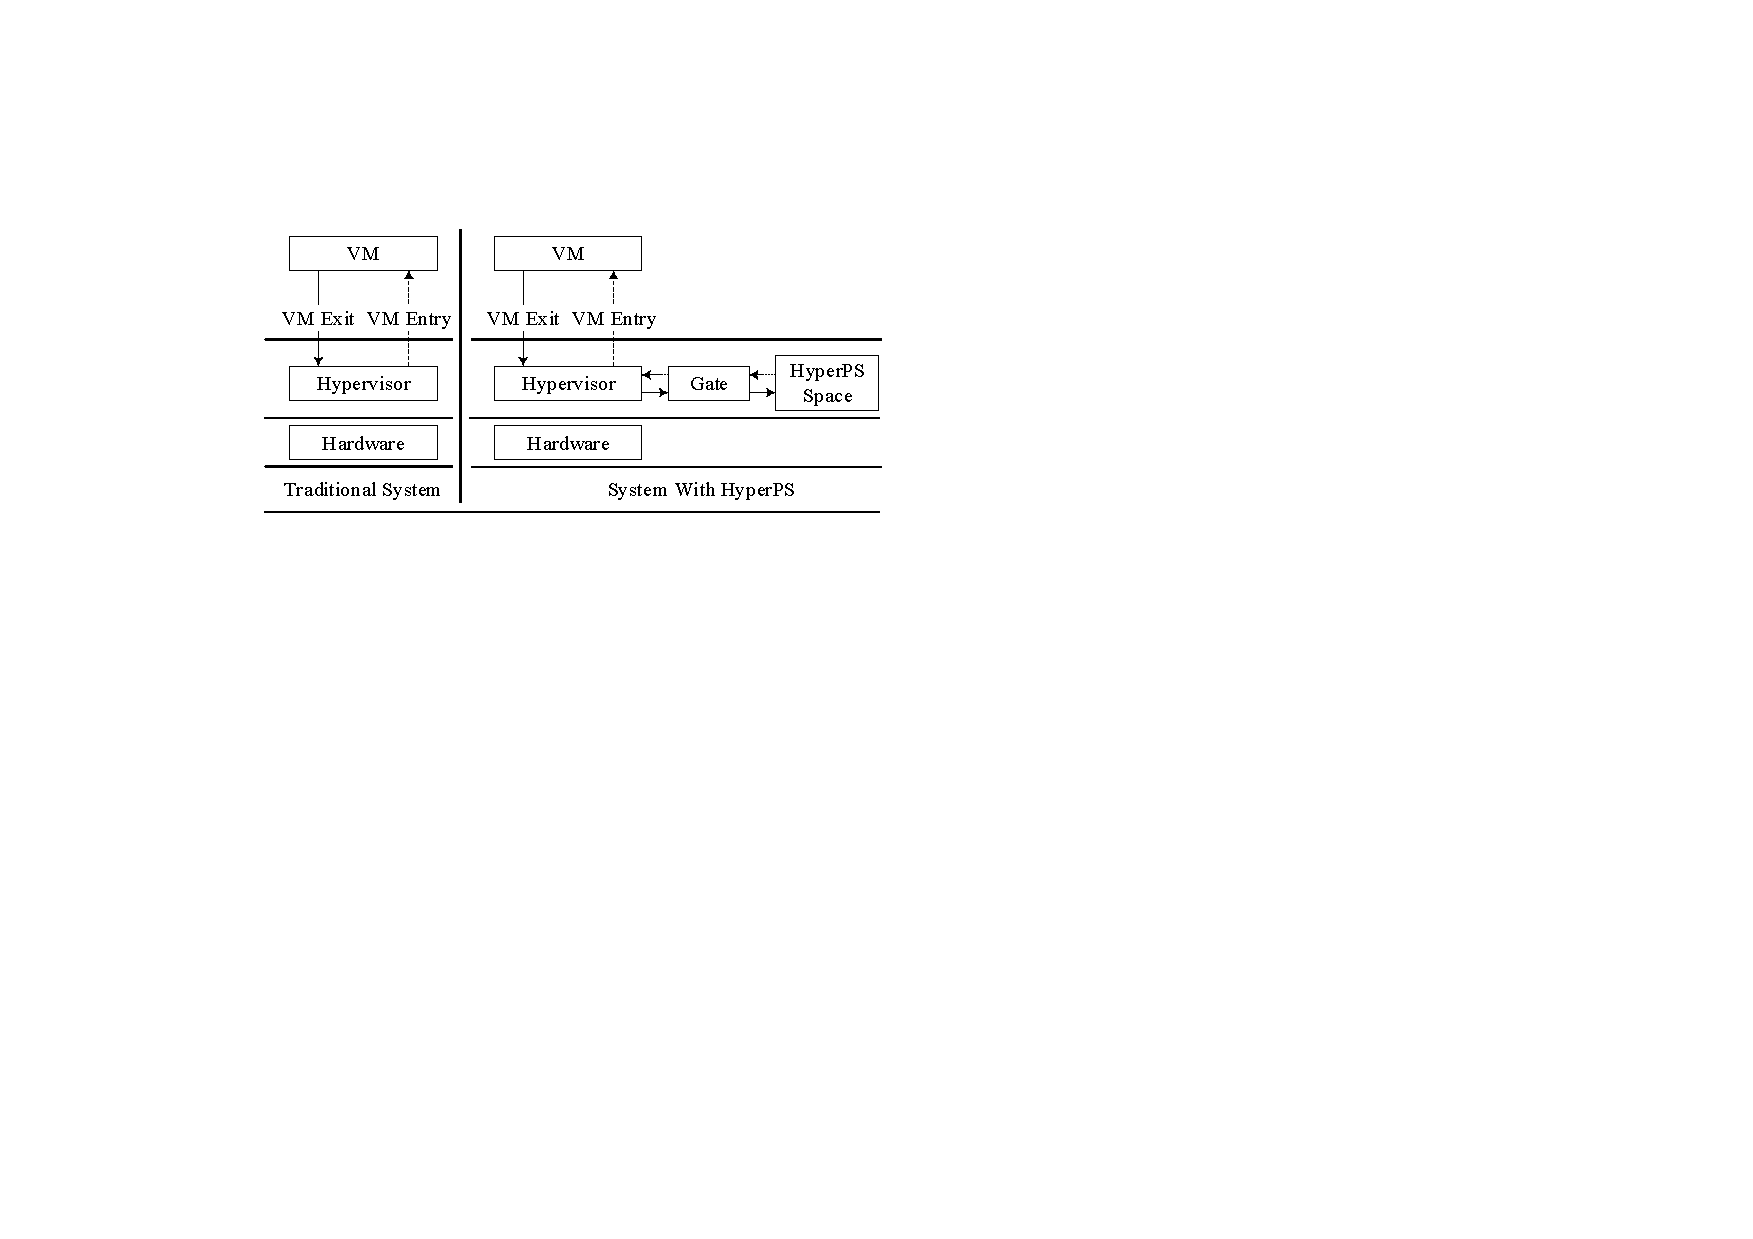
\includegraphics[width=0.8\linewidth]{IMG/interaction.pdf}
    \caption{Interaction Difference between the traditional system and system with HyperPS \\ VM-Exit handling only involves the hypervisor in traditional system. In the system with HyperPS, VM-Exit is redirect into the HyperPS Space through the Gate. Context Management during VM-Exit and VM-Entry is managed by the HyperPS.}%
    \label{fig:inter}
\end{figure}


% Exception handle
% all code and any data in guest
% any VM's content in memory can no longer be
% EPT paging structures
% neither isolation between VMs nor virtual-physical mapping relationships in a VM
% nor
% In this paper, HyperPS deprives the compromised hyperivor with privileges of managing physical memory by limiting it from accessing and managing all EPTs.
% deprives the virtual machine
% 上面的内容说明了要限制权限是通过EPT来实现的。怎么移除EPT 为什么要移除VMCS
\iffalse
首先要讲管理内存的权限是通过EPT实现的,要实现特权的分离,分为两步,一是将EPT从原有空间移除,使得原有的hypervisor无法直接access数据结构。第二步是对能access这些数据结构的函数进行验证。
% 将移除操作这些数据结构的逻辑。
在传统的没有HyperPS的虚拟化环境中,Hypervisor 通过EPT直接管理管理内存
这里要先讲为什么要将EPT和VMCS从原有的空间移除,然后再讲怎么移除。移除以后存在疑问,就是会造成PANIC, 如何解决,就是hook的问题,
It's EPT mechanism that treat guest-physical address like a virtual address and the EPTP is the CR3.
we should write (VMWRITE) EPTP to the VMCS. 
\fi


Firstly, HyperPS removed all EPTs and VMCSs from the hypervisor space. EPT manages all physical memory of the VM, as mentioned above, HyperPS removed themfrom the hypervisor space. However, there is a hardware register, called Extended Page Table Pointer (EPTP), that contains the address of the base of EPT table, as well as EPT configuration information. Simple obliteration of EPT would make EPTP error which will crash the whole virtualization environment too. 
Besides, the VMCS records the value of EPTP in the VM-Execution Control Fields. The processor will load the value in that field into the hardware register when VM-Entry. 
Even if the attacker cannot directly tamper the EPT, he can also subvert the guest VMs by tampering with a malicious EPTP value in the VMCS. Thus, HyperPS removed all VMCSs from the hypervisor too. 
% The adversary can tamper with the EPTP value in the VMCS to make the VM use a new set of malicious EPT table.
% Thus, HyperPS
% A hypervisor load the value
% EPTP is a hardware register that works like the CR3 register in traditional memory translation. It always points to the
% The VMCS stores the value of EPTP in the VM-Execution Control Fields.
% VMCS store EPTP that points to EPT
% EPTP works like the CR3 in

Secondly,  HyperPS hooks all VMCS operation and EPT operation functions in the hypervisor into the HyperPS space.
Based on Intel manuals, VMCS can only be manipulated by privileged instructions: \verb|VMCLEAR| \verb|VMPTRLD|, \verb|VMREAD|, \verb|VMWRITE|, and so on.
In the QEMU-KVM architecture, the KVM is responsible for executing these privileged instructions. The KVM provdes a wrapper around these privileged instructions. The QEMU does not need to deal architecture specific details, it just need to invoke KVM functions with proper parameters. 
For example, \verb|vmcs_writel()| wraps the privileged instruction \verb|VMWRITE|, and \verb|vmcs_readl()| wraps the privileged instruction \verb|VMREAD|.
HyperPS hooks these functions into the HyperPS space. In the HyperPS space, Context Management in the HyperPS Space Management component check the invoked parameters and verifies if the write to \verb|VM-Execution Control Fields.EPTP| is legal or not. 
Since VMCS is hidden in the HyperPS space which is unaccessable by functions in the hypervisor space, all context management (accessing VMCS operations) must be trapped to HyperPS space. 
%During VM-Exit (codes to access VMCS can only be executed in VM-Exit), the hypervisor 
EPT operation functions are also hooked into the HyperPS Space too. EPT operation functions are different with VMCS operation functions, for the VMCS can only be accessed by just a few privileged instructions. Instead of hooking EPT accessing functions, HyperPS hooks all EPT operation functions. Functions about EPT creation, load, iteration, and destroy are re-place them into the HyperPS space. Functions invoke these EPT operation functions are hooked into the HyperPS Space.

% operation functions
% HyperPS checks the
% provide a wrapper around these privileged instructions.
% are responsible
% HyperPS hooks functions that contain these instructions.
% In specific,
% at each time when VM exits to the hypervisor, HyperPS
% VMCS operation and EPT operation functions certainly involve privileged instructions.
% On a privileged instruction, it switches back to the KVM kernel module,

Lastly, HyperPS also takes DMA attacks into consideration. An attacker with the ability of arbitrary memory access by exploiting DMA vulnerabilities can tamper VMCSs and EPTs. IOMMU carries out access control for DMA access. Thus, in this paper, HyperPS employs IOMMU mechanism to resist DMA attacks.
In the hypervisor space, HyperPS found out all the critical data used by IOMMU, and removed the corresponding page table entries that map these data from the page tables. In this paper, HyperPS mainly defines the entrance address of HyperPS, the Page-Mark data, and the VM-Mark data (details about Page-Mark and VM-Mark data structure are illustrated in Section \ref{sub:vm_memory_protection}) as the critical data.
In the HyperPS space, HyperPS intercepts the address mapping function about I/O. At runtime, HyperPS verifies whether the address belongs to the HyperPS space on receiving signals of executing these IO functions. 


% HyperPS removed all corresponding page table entries that map
% mapping of the critical data from the page table which IOMMU uses.
% In the HyperPS Space, DMA Management Component
% In this paper, HyperPS employs IOMMU mechanism to resist DMA attacks. IOMMU carries out access control for DMA access.

\subsection{VM Memory Protection}%
\label{sub:vm_memory_protection}























